\documentclass{aa}
\usepackage[T1]{fontenc}
\usepackage{lmodern}
\usepackage{graphicx,amsmath,amssymb,booktabs,tabularx}
% Hyperlinks omitted for compatibility with the bundled A&A class.
\newcommand{\Tinf}{\widetilde T}
\newcommand{\Msun}{M_\odot}
\begin{document}
\raggedbottom
\title{Neutron-star cooling revisited}
\subtitle{Microphysical prescriptions, thermal envelopes, and observational interpretation}
\author{Author list to be agreed}
\institute{Affiliations to be completed}
\date{Working draft updated 19 November 2026}
\abstract
{Thermal emission from isolated neutron stars probes dense matter through a combination of stellar structure, neutrino emission, heat capacity, transport, and surface boundary conditions. Many calculations still combine prescriptions developed at different times and within different microscopic approximations.}
{We reassess non-magnetic cooling from the benchmarks established by Yakovlev et al. (2001) and Page et al. (2004), using Aguilera et al. (2008) as an implementation-era reference. We distinguish corrections to established expressions from competing physical models and from numerical implementation choices.}
{We compare published prescriptions for nucleonic and leptonic processes, superfluidity, thermal conductivity, and heat-blanketing envelopes, and examine the assumptions linking cooling predictions to observations. Detailed derivations are referred to the original literature.}
{The principal developments concern the weak response of paired matter, the nuclear interaction and intermediate states entering neutrino reactions, consistent composition and effective masses, and the treatment of envelope composition and observational systematics. These developments do not define a single multiplicative update to an older cooling model. They affect different density and temperature regimes, and some cannot be combined without double counting.}
{A useful modern benchmark must specify a coherent set of assumptions and expose alternatives explicitly. Observational claims about enhanced cooling should survive variations in pairing, envelope composition, source age, and spectral interpretation. Preliminary matched-star calculations demonstrate EOS-dependent sensitivity to gap amplitudes and connect integrated neutrino dominance to local emissivity profiles. A systematic comparison of competing microphysical prescriptions and a source-by-source observational catalogue remain to be completed.}
\keywords{stars: neutron -- dense matter -- neutrinos -- conduction -- radiation mechanisms: thermal}
\maketitle

\section{Introduction and scope}
The reviews of \citet{Yakovlev2001} and the minimal-cooling study of \citet{Page2004} provide complementary starting points. The former establishes a practical inventory of neutrino reactions; the latter asks whether an explicitly restricted set of processes can account for observed thermal emission. Their value lies as much in making assumptions identifiable as in providing formulae. A comparison described simply as ``standard cooling'' can otherwise conceal different particle populations, pairing models, or surface boundary conditions.

\citet{Aguilera2008} assembled detailed microphysics within a two-dimensional thermal calculation. Here we retain the underlying cooling problem but exclude magnetic transport, field evolution, and Joule heating. This restriction permits a clearer assessment of non-magnetic ingredients; it does not imply that magnetic effects are negligible for every observed neutron star. The later syntheses of \citet{YakovlevPethick2004,Potekhin2015,Schmitt2018} provide the broader context.

The intervening literature has not merely replaced old coefficients with better ones. Some developments repair approximations that violate a conservation law; others change the nuclear interaction or the quasiparticle spectrum; still others reveal that the data admit several astrophysical interpretations. We therefore use three categories throughout: an identifiable implementation error, a controlled improvement within a specified approximation, and an alternative physical prescription. Only the first category can normally be resolved without considering the wider model.

Our primary domain is an isolated, slowly rotating, neutrino-transparent star with nucleonic matter and electrons and muons. We discuss additional constituents and heating as limitations of this domain, rather than attempting a complete review of exotic cooling. The first draft is a critical synthesis, not a new measurement of nuclear parameters. In particular, no new exclusion of an equation of state (EOS) is inferred from the present numerical implementation.

\section{Stellar structure and thermal evolution}
\subsection{Redshifted quantities and the cooling problem}
On a static spherical background, thermal equilibrium corresponds to a spatially constant redshifted temperature, $\Tinf=e^\Phi T$, rather than a constant local temperature. For a uniform surface, the observed thermal luminosity is
\begin{equation}
 L_\gamma^\infty=4\pi R^2\sigma T_s^4 e^{2\Phi_s},
 \qquad T_s^\infty=e^{\Phi_s}T_s.
\end{equation}
We follow the relativistic thermal-evolution conventions reviewed by \citet{YakovlevPethick2004}. The familiar global balance,
\begin{equation}
 C(\Tinf)\frac{d\Tinf}{dt}=-L_\nu^\infty-L_\gamma^\infty+H^\infty,
\end{equation}
is appropriate after the interior becomes approximately isothermal in $\Tinf$. It must not replace spatial heat transport during crust--core relaxation. In the passive models considered here $H^\infty=0$; this is a model assumption, not a statement about all old neutron stars.

A static cold background is usually adequate once thermal corrections to pressure are small. Very early evolution requires greater care with both the EOS and the quasi-stationary envelope approximation. \citet{Potekhin2018} demonstrate the relevance of resolving the outer layers when extending calculations to short times. An arbitrary hot initial profile is therefore not a prediction for the proto-neutron-star cooling stage.

\subsection{Composition and effective masses must belong to a specified model}
A unified EOS reduces ambiguities associated with joining independently constructed crust and core models. The Brussels--Montreal family provides an instructive example: related functionals yield different compositions and high-density behaviour \citep{Pearson2018}. Similar radii do not ensure similar cooling, because the proton and lepton fractions determine reaction thresholds.

For charge-neutral nucleonic matter, $n_p=n_e+n_\mu$. Replacing $n_p$ by $n_e$ after muons appear changes both kinematics and rate normalisations. It is likewise insufficient to import only a pressure--density table and obtain the particle fractions from an unrelated approximation. A reproducible model should supply the background, composition, and any available quasiparticle information together.

The effective mass required by a degenerate heat-capacity or phase-space expression is tied to the density of states at the Fermi surface. It is not automatically the Dirac mass of a relativistic mean-field model. \citet{Schmitt2018} discuss this quasiparticle description and its relation to transport. Our consistency criterion is consequently more specific than ``use effective masses'': identify their definition and source, then use them consistently wherever that definition is appropriate. Replacing mass prefactors alone does not convert an interaction model into a different many-body theory.

\section{Heat capacity and pairing}
\subsection{The thermal reservoir}
Degenerate electrons, muons, and normal nucleons provide approximately linear-in-temperature contributions to the heat capacity. Pairing changes the nucleonic terms near the transition and suppresses them at lower temperatures; the ionic contribution changes across the liquid and crystalline regimes. The classic treatment of \citet{Yakovlev1999} remains a useful reference for the thermal consequences of pairing.

The main question is not which species has the largest normal-state coefficient, but which remains thermally active along the evolving profile. After strong nucleonic suppression, leptons can control the heat reservoir. Muons should therefore enter the heat capacity even in a model where their neutrino channel is kinematically closed. In the crust, the heat capacity of unbound neutrons cannot be assessed independently of their pairing state.

\subsection{Gap models are not interchangeable fit functions}
The fitted gap catalogue used by \citet{Ho2015} is useful for comparing the consequences of different microscopic calculations. A fit, however, preserves a selected calculation rather than establishing a probability distribution over physically allowed gaps. Its density support, maximum critical temperature, and high-density closure are all relevant. The study of \citet{Ding2016} illustrates how short- and long-range correlations alter the underlying pairing problem.

A controlled comparison should change a gap model simultaneously in the heat capacity, the suppression of ordinary neutrino reactions, pair breaking and formation (PBF), and the appropriate transport coefficients. Changing only a PBF curve is a sensitivity experiment on that channel, not a self-consistent change of superfluidity. The gap amplitude, the critical temperature, and the dimensionless quantity used in reduction functions must also follow one convention, especially for anisotropic triplet pairing.

Superfluidity does not invariably accelerate cooling. It can reduce neutrino losses, produce a transient PBF contribution, and remove heat capacity. Their relative importance changes with age. The conclusions of \citet{Page2009} about minimal cooling are conditional on the range of critical temperatures present in the core and on heterogeneous envelope compositions. They should not be promoted to a universal preference for one gap amplitude.

\section{Neutrino emission: competing prescriptions}
\subsection{Direct Urca and the role of muons}
The direct-Urca mechanism introduced into neutron-star cooling by \citet{Lattimer1991} changes the interpretation of composition dramatically: a modest change in proton fraction can open a powerful channel. In the strongly degenerate, zero-temperature kinematic limit, each lepton branch requires $p_{Fn}\leq p_{Fp}+p_{F\ell}$, with $\ell=e,\mu$. The thresholds are separate; neither a fixed proton-fraction threshold nor a factor of two applied to the electron rate is generally sufficient.

The standard expressions and lepton substitutions are collected in Sect.~3.3 of \citet{Yakovlev2001}. Their $T^6$ scaling contrasts with the $T^8$ scaling of modified Urca in the normal, degenerate regime. Pairing and finite-temperature threshold broadening qualify this simple distinction. Numerically, the volume of the allowed region also matters: a coarse grid can turn a small central emitting region on or off abruptly. Threshold convergence should be checked before interpreting a sharp mass dependence as physical.

\subsection{Modified Urca: define the reference before quoting a correction}
The calculation of \citet{Friman1979} is a historical foundation for both modified Urca and nucleon bremsstrahlung. It combines a model of the nuclear interaction with approximations to the reaction kinematics. Later practical formulae are not all identical transcriptions of it. The prescription of \citet{Yakovlev1995}, for example, and the benchmark collected by \citet{Yakovlev2001} must be labelled separately. Density-dependent interaction factors, proton-branch phase space, effective-mass conventions, and the treatment of the muon branch can all differ.

This distinction matters when rates are compared as a ratio to ``Friman--Maxwell''. The denominator must be an explicit expression with stated assumptions. A ratio obtained by removing a density-dependent factor from an existing implementation answers a useful diagnostic question, but it is not automatically a comparison with the original paper. Likewise, a constant enhancement of both branches is a phenomenological experiment; it does not reproduce the density dependence of a microscopic correction.

For a conventional benchmark we favour the explicitly identified normal-state expressions in Eqs.~(140)--(142) of \citet{Yakovlev2001}, with both lepton branches and the stated phase-space restrictions. This is a reference for comparison, not a claim that the interaction physics is final. Superfluid reductions must be attached with their own provenance; the work of \citet{Gusakov2002} is particularly relevant when more than one paired component or an anisotropic gap is involved.

\subsection{Revised interaction calculations and medium enhancements}
\citet{Bottaro2024} revisit the interaction framework underlying the traditional rates, reassessing exchange and interference contributions and the triangular approximation. Their published normal-state results provide a valuable alternative benchmark. However, a numerical implementation retaining only their leading approximations should not be described as implementing their complete angular treatment. Effective-mass substitutions and superfluid reductions subsequently attached to those rates are additional assumptions.

A different development is the enhancement found by \citet{Shternin2018}, associated with the in-medium spectrum of the intermediate nucleon as the direct-Urca threshold is approached from below. Their practical approximation concerns the neutron branch and has a stated domain of applicability. This is not a uniform rescaling of all modified-Urca channels. Its threshold behaviour also warns against extrapolating a perturbative expression through a region where its underlying approximation ceases to be controlled.

The nuclear-medium cooling approach exemplified by \citet{Blaschke2004} explores a broader, correlated set of medium-dependent ingredients. Its interpretation should be compared with minimal cooling at the level of complete model families. Pion softening, vertex changes, and pairing assumptions should not be silently compressed into one universal enhancement coefficient.

Our recommendation is to compare these alternatives separately before attempting a hybrid. A fitted medium-enhancement factor can already contain the normalisation of its own scattering model. Multiplying it by an independently revised interaction rate can count some effects twice. Constructing a combined prescription would require identifying their shared approximation and matching the relevant contributions; agreement at one density is insufficient.

\subsection{Nucleon bremsstrahlung}
The $nn$, $np$, and $pp$ channels involve different interaction and symmetry factors. The standard normalisations are given in Eqs.~(165)--(167) of \citet{Yakovlev2001}; neutrino-flavour multiplicity must be counted once. Distinguishing this bookkeeping from physical uncertainty is essential: a duplicated flavour factor is an error, whereas a different scattering amplitude is a model choice.

The effective-interaction calculation of \citet{Schwenk2004} and the later reassessment by \citet{Bottaro2024} illustrate that corrections to a pion-exchange benchmark need not increase the rate. Short-range suppression factors inherited from an older formula must be examined before being retained in a new one. Their numerical value and original purpose should be recorded explicitly. A revised rate should be compared both before and after any legacy multiplier, so that its effect is not attributed incorrectly to the new calculation.

Bremsstrahlung may become important when Urca channels are suppressed, but local emissivity comparisons alone do not establish global dominance. The density volume, temperature profile, and pairing state must enter the luminosity integral. This is also why a change in a subdominant local channel can be negligible for one star and relevant for another.

\subsection{Pair breaking and formation: conservation and axial vertices}
\label{sec:pbf-response}
Early PBF rates require revision because an inconsistent vector response can violate current conservation. \citet{Leinson2006} showed the strong suppression of the vector contribution for singlet-paired baryons. This correction is conceptually different from changing a fitted gap. \citet{Page2009} demonstrated that axial emission still permits efficient PBF cooling within the minimal scenario.

Removing the vector term does not complete the triplet problem. \citet{Leinson2010} includes anomalous weak vertices and obtains a further change in the triplet response. Thus ``vector-corrected PBF'' and ``PBF with anomalous axial vertices'' must not be used as synonyms. \citet{Potekhin2018} incorporate the latter developments in their microphysics discussion. Comparisons of numerical coefficients should be made only after matching the definitions of the angular function, the gap amplitude, and the weak-coupling factors.

The defensible hierarchy is to retain current conservation, state the adopted triplet phase and response approximation, and vary the gap separately from the weak vertex. A single freely adjustable PBF normalisation may be informative phenomenologically, but does not identify the microscopic origin of the discrepancy. Nor should a coefficient for neutral neutron matter be transferred without qualification to superconducting protons embedded in a charged plasma.

\subsection{Crustal and thermal processes}
Electron--ion bremsstrahlung remains an essential crustal process. \citet{Kaminker1999} account for the properties of the Coulomb medium, including the crystalline regime, rather than treating all ions as independent scattering centres. The thermal processes tabulated by \citet{Itoh1996}, including pair annihilation and plasmon decay, supply complementary contributions where their thermodynamic assumptions apply.

These channels deserve the same transcription discipline as core rates. A logarithm base, a temperature unit, or a swapped digit in a prefactor can produce an apparent physical disagreement. Repairing such an error should precede an interpretation in terms of new medium physics. Conversely, agreement of a fit with its source does not demonstrate validity outside its density, composition, and degeneracy domain.

\begin{table*}
\caption{Prescriptions to distinguish in a modern comparison. ``Benchmark'' does not mean uniquely preferred physics.}
\label{tab:rates}
\centering\small
\begin{tabularx}{\textwidth}{p{2.4cm}p{3.7cm}X}
\toprule
Ingredient & Reference family & Critical distinction \\
\midrule
Modified Urca & \citet{Friman1979,Yakovlev1995,Yakovlev2001} & Identify the actual formula, composition, branch phase space, and mass conventions; the historical labels are not interchangeable.\\
Revised nuclear amplitudes & \citet{Bottaro2024} & Separate leading kinematic approximations from the more general angular treatment and from added legacy factors.\\
Medium-modified Urca & \citet{Shternin2018,Blaschke2004} & Different medium approximations are not universal correction factors; threshold extrapolation requires control.\\
Bremsstrahlung & \citet{Schwenk2004,Bottaro2024} & Interaction corrections, symmetry factors, flavour counts, and superfluid reductions are distinct operations.\\
PBF & \citet{Leinson2006,Page2009,Leinson2010} & Vector-current suppression and anomalous axial vertices are separate developments; gap uncertainty is a third issue.\\
Pairing reductions & \citet{Yakovlev1999,Gusakov2002} & Match the process, participating species, and pairing symmetry rather than multiplying arbitrary one-species factors.\\
\bottomrule
\end{tabularx}
\end{table*}

\section{Thermal conductivity}
\subsection{Core transport}
The electron--muon calculation of \citet{Shternin2007} incorporates transverse electromagnetic interactions and the effect of proton superconductivity on screening. It is not equivalent to duplicating an electron conductivity with the muon mass substituted. The carriers participate in a coupled collision problem, even though their contributions to the total heat current can ultimately be separated. The neutron contribution has its own interaction and pairing dependence \citep{Baiko2001}.

The transport review of \citet{Schmitt2018} makes clear why consistency requires more than using the same effective masses in every prefactor. Collision amplitudes and screening must be specified as well. A simplified lepton prescription can be retained for a controlled comparison, but it should be labelled as an approximation rather than attributed to the full coupled calculation.

\subsection{Crust transport and justified simplification}
The treatment of \citet{Potekhin1999} provides an established basis for electron transport across liquid and solid regimes. Electron--electron collisions can also matter, particularly where other scattering mechanisms are weak \citep{Shternin2006}. Impurity scattering introduces a dependence on the charge distribution that is not determined by a single representative nucleus. A chosen impurity parameter should therefore remain identifiable as a model input.

For a cold, degenerate, non-magnetic interior, a restricted conductivity implementation may be much simpler than a general-purpose routine. The restriction should be defined physically: degeneracy, phase, composition, and the density of the outer boundary. It should not be justified by the calendar year in a routine filename. Non-degenerate surface layers still require their own conductive and radiative treatment. The effects of a simplification must be assessed during thermal relaxation, when heat transport has its strongest leverage, as well as along the later cooling curve.

\section{Heat-blanketing envelopes and surface emission}
\subsection{From iron fits to composition-dependent blankets}
\citet{Gudmundsson1983} established a widely used relation between the temperature at the base of an iron envelope and the effective surface temperature. It remains a useful reference, provided its gravity convention, base density, and applicability range are retained. The envelope is a boundary model for unresolved layers, not a freely interchangeable conversion between arbitrary interior and surface temperatures.

\citet{Potekhin1997} showed the importance of accreted light elements. Their insulating properties differ from those of a heavy-element blanket, so that two stars with the same internal temperature can have different surface luminosities. The resulting cooling histories cannot be understood as a fixed vertical offset: enhanced photon losses also change the later internal evolution.

Diffusive mixtures further refine the composition problem \citep{Beznogov2016}. The synthesis by \citet{Beznogov2021} treats layered and mixed envelopes, diffusion, and high-temperature limitations. For practical comparisons, the mass or column of light elements should be a parameter. Pure iron and fully accreted endpoints are informative, but do not sample the full uncertainty. Chemical survival and burning also limit which assumed blankets are physically plausible at a given age.

\subsection{The atmosphere is a different physical layer}
The envelope controls the relation between interior heat and the outgoing flux. The atmosphere determines the emergent spectrum from which observers infer temperature, emitting area, and bolometric luminosity. A thin hydrogen atmosphere does not establish that a thermally important hydrogen-rich blanket extends to the chosen envelope base. Conversely, an iron-envelope calculation is not a justification for fitting an observed spectrum with a blackbody.

The catalogue of \citet{Potekhin2020} illustrates the dependence of inferred thermal quantities on spectral assumptions. Model--data comparisons should use compatible definitions of luminosity and redshift and preserve alternative spectral solutions when the observations do not discriminate among them. Fitted colour temperatures and effective temperatures should not be placed on the same cooling diagram without the corresponding interpretation.

\subsection{Boundary implementation}
For an implicit heat solver, the surface flux and its derivative must be computed from the same envelope relation. Any fit replacement changes both. The derivative is a numerical ingredient, not an additional physical correction to the emergent luminosity. A consistent implementation also distinguishes the radius of the computational boundary from the stellar photospheric radius. These conventions can be documented without reproducing lengthy fitting expressions in the main text.

\section{Numerical verification and a reproducible comparison}
The purpose of the numerical implementation is to expose physical alternatives without changing unrelated assumptions. We propose three successive levels: reproduce the cited local expressions; demonstrate energy balance and spatial and temporal convergence; then compare complete cooling histories. Agreement with an older code tests a translation, but cannot establish that the older prescription was physically correct.

The independent energy ledger must use the internal energy obtained by integrating the heat capacity, not $C_VT$ in place of that integral. Neutrino emissivities and photon luminosities must carry consistent redshift factors. Windowed closure errors are useful during thermal relaxation because an accumulated residual can be dominated by an unresolved initial stage. Temperature-change control is an adaptive step criterion, not a guaranteed bound on energy error.

The present working implementation provides a spherical framework, composition-dependent lepton populations, modular microphysics, and implicit envelope boundary conditions. Its current choices are not uniformly the most complete literature treatments. In particular, the documented simplified lepton transport and retained PBF response require dedicated comparisons. These limitations should remain visible in a publication even if their effect proves small for the reference star.

\subsection{Comparison programme}
A useful first sequence holds the EOS, stellar mass, gap models, envelope, grid, and integration tolerance fixed while replacing one prescription. A second sequence varies physically connected ingredients together. Effective masses, gap models, and collision amplitudes should not all be described as independent uncertainties if they originate in the same microscopic theory.

The proposed figures are: normal-state emissivities and their ratios along common density profiles; paired emissivities and heat capacities over selected temperatures; competing envelope relations; cooling curves with matched assumptions; and a final comparison with the observational sample. The luminosity of each neutrino process should be integrated over the star. A local emissivity maximum does not identify the process governing the global cooling rate. The following first comparisons implement part of this programme; no quantitative exclusion of an EOS or gap model is inferred.


\subsection{Matched reference stars and EOS dependence}
\label{sec:numerical-results}
We now implement a first controlled sequence with BSk22, BSk24, BSk25, BSk26, and DDFGOS(APR). Each star has a target gravitational mass of $1.4\,\Msun$, with its central pressure determined independently from its EOS. The cold structure, composition, and tabulated Landau effective masses are used together. All calculations have $B=0$, no heating, a Gudmundsson envelope, and an initially uniform redshifted temperature of $10^{10}$ K. The reference uses the implemented Yakovlev et al.\ modified-Urca prescription and Bottaro et al.\ nucleon bremsstrahlung, together with the other registered channels. These are named working choices, not a recommendation that their combination is a unique microscopic model \citep{Yakovlev2001,Bottaro2024}.

The mesh-C prescription is used throughout; it defines EOS-dependent meshes under common resolution rules, rather than identical radial points. The predictor--corrector integration uses a maximum accepted relative temperature change of 1.25\%, with the first 20 steps fixed at 0.01 yr. Runs stop at their first accepted $L_\gamma^\infty<10^{31}$ erg s$^{-1}$; no continuation below this cutoff is inferred. The retained reference PBF response is the one discussed in Sect.~\ref{sec:pbf-response}: varying gaps below does not change its weak-vertex prescription. Numerical energy closure does not validate that physical response or establish spatial convergence.

Figure~\ref{fig:five-eos} compares the five reference stars. Changing the EOS changes structure, composition, effective masses, reaction thresholds, and the portion of the fitted gap sampled by the star. Consequently, this comparison does not isolate any one of those effects. The handling of the BSk25 and BSk26 pressure inversions and the existing APR density discontinuity is specified in Appendix~\ref{app:eos-tables}. DDFGOS(APR) denotes the particular CompOSE reconstruction used here, not every EOS commonly called APR. Its unresolved inner-crust composition mapping leaves the corresponding crustal heat capacity and transport provisional.

\begin{figure*}[t]
\centering
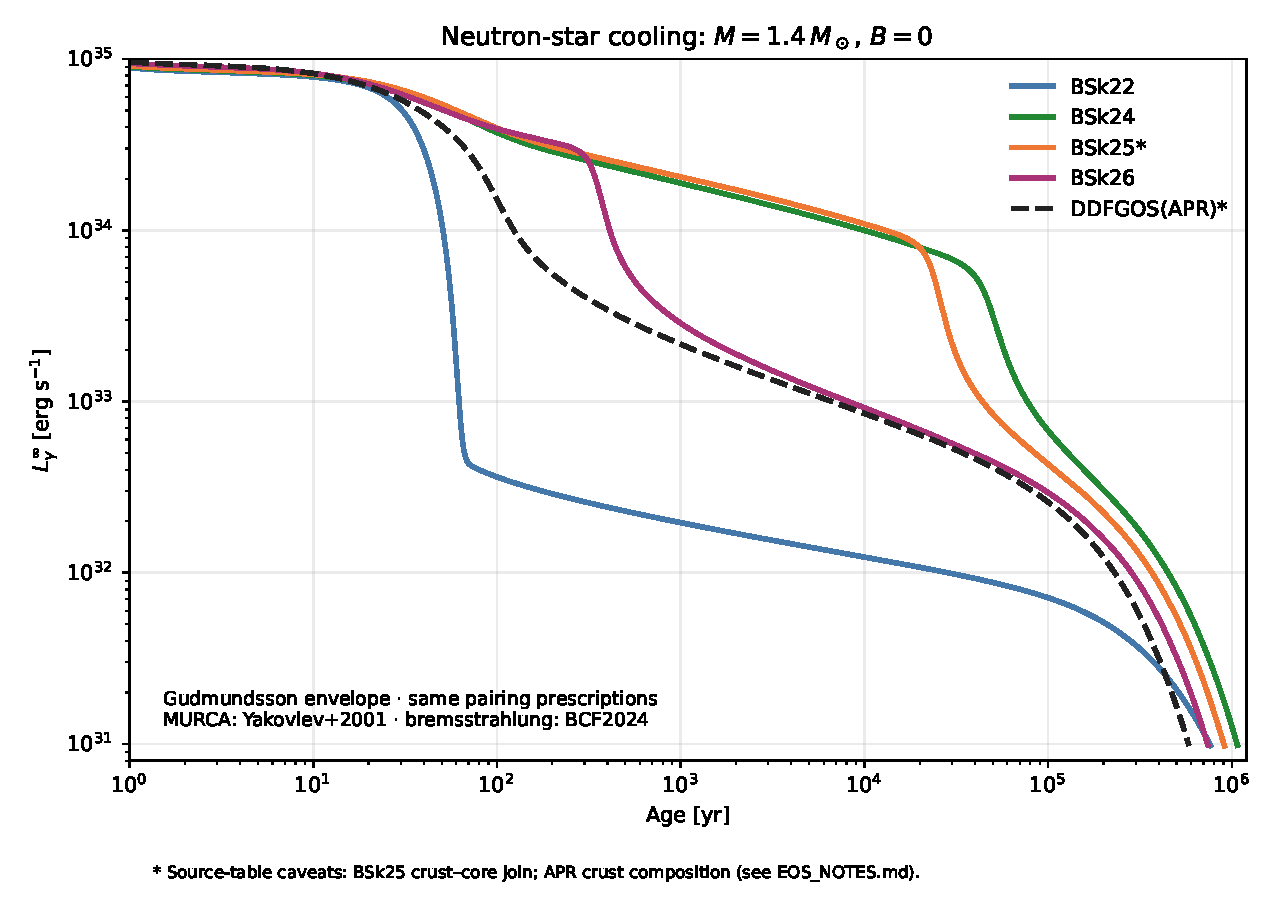
\includegraphics[width=0.82\textwidth]{figures/cooling_five_eos.pdf}
\caption{Reference photon luminosities at infinity for five EOSs at a common target mass of $1.4\,\Msun$. Pairing prescriptions, envelope, integration controls, and mesh prescription are common. BSk25 uses the adopted discrete crust--core connection; the APR crust-composition caveat remains. Differences include EOS-dependent sampling of the same gap functions and, where allowed, direct Urca. These curves are model comparisons, not fits to observations.}
\label{fig:five-eos}
\end{figure*}

\subsection{Controlled variation of gap amplitudes}
\label{sec:gap-scan}
For BSk24 and DDFGOS(APR), we construct the background once per EOS and hold it fixed while changing one pairing channel at a time. The reference fits are the crustal neutron singlet, proton singlet, and deep core-neutron triplet fits used by the working implementation and discussed alongside the catalogue of \citet{Ho2015}; their implementation catalogue numbers are 7, 8, and 12, respectively. These numbers identify code entries, not universal model names. The triplet conversion retained here is $k_BT_c/\Delta_B=0.8416$, while the singlet conversion is 0.5669. The precise five-parameter tuples are archived with the calculation.

For each of the three channels, we apply
\begin{equation}
 T_{c,i}(\rho_b)\longrightarrow s\,T_{c,i}(\rho_b),
 \qquad s=0,\;0.5,\;2,
\end{equation}
while the other channels retain $s=1$. Here $\rho_b=(1.66\times10^{-24}\,{\rm g})n_b$ is the baryon mass-density convention of the microphysics. Scaling $T_c$ is equivalent to scaling the fitted gap amplitude at fixed conversion factor. Both cell and face values are changed, and the resulting temperatures enter the heat-capacity, emissivity, and transport evaluations. The momentum support and shape of each gap remain fixed. This gives one reference and nine variations per EOS, rather than a Cartesian scan of all three amplitudes. The $s=0$ case switches off that pairing channel; it is a limiting diagnostic, not a preferred microscopic calculation.

Figures~\ref{fig:gap-curves} and \ref{fig:gap-ratios} show that the response is neither independent of the EOS nor uniformly monotonic with amplitude at a fixed age. Varying the crustal gap by factors of two mainly changes the early relaxation. Core-neutron pairing produces much larger changes, with an EOS-dependent onset and duration. Proton-gap changes have a sustained effect in BSk24 but are concentrated at early ages in APR for the nonzero factors considered here. Removing proton pairing entirely also changes the late thermal reservoir, so its effect need not have the same sign at all ages.

\begin{figure*}[t]
\centering
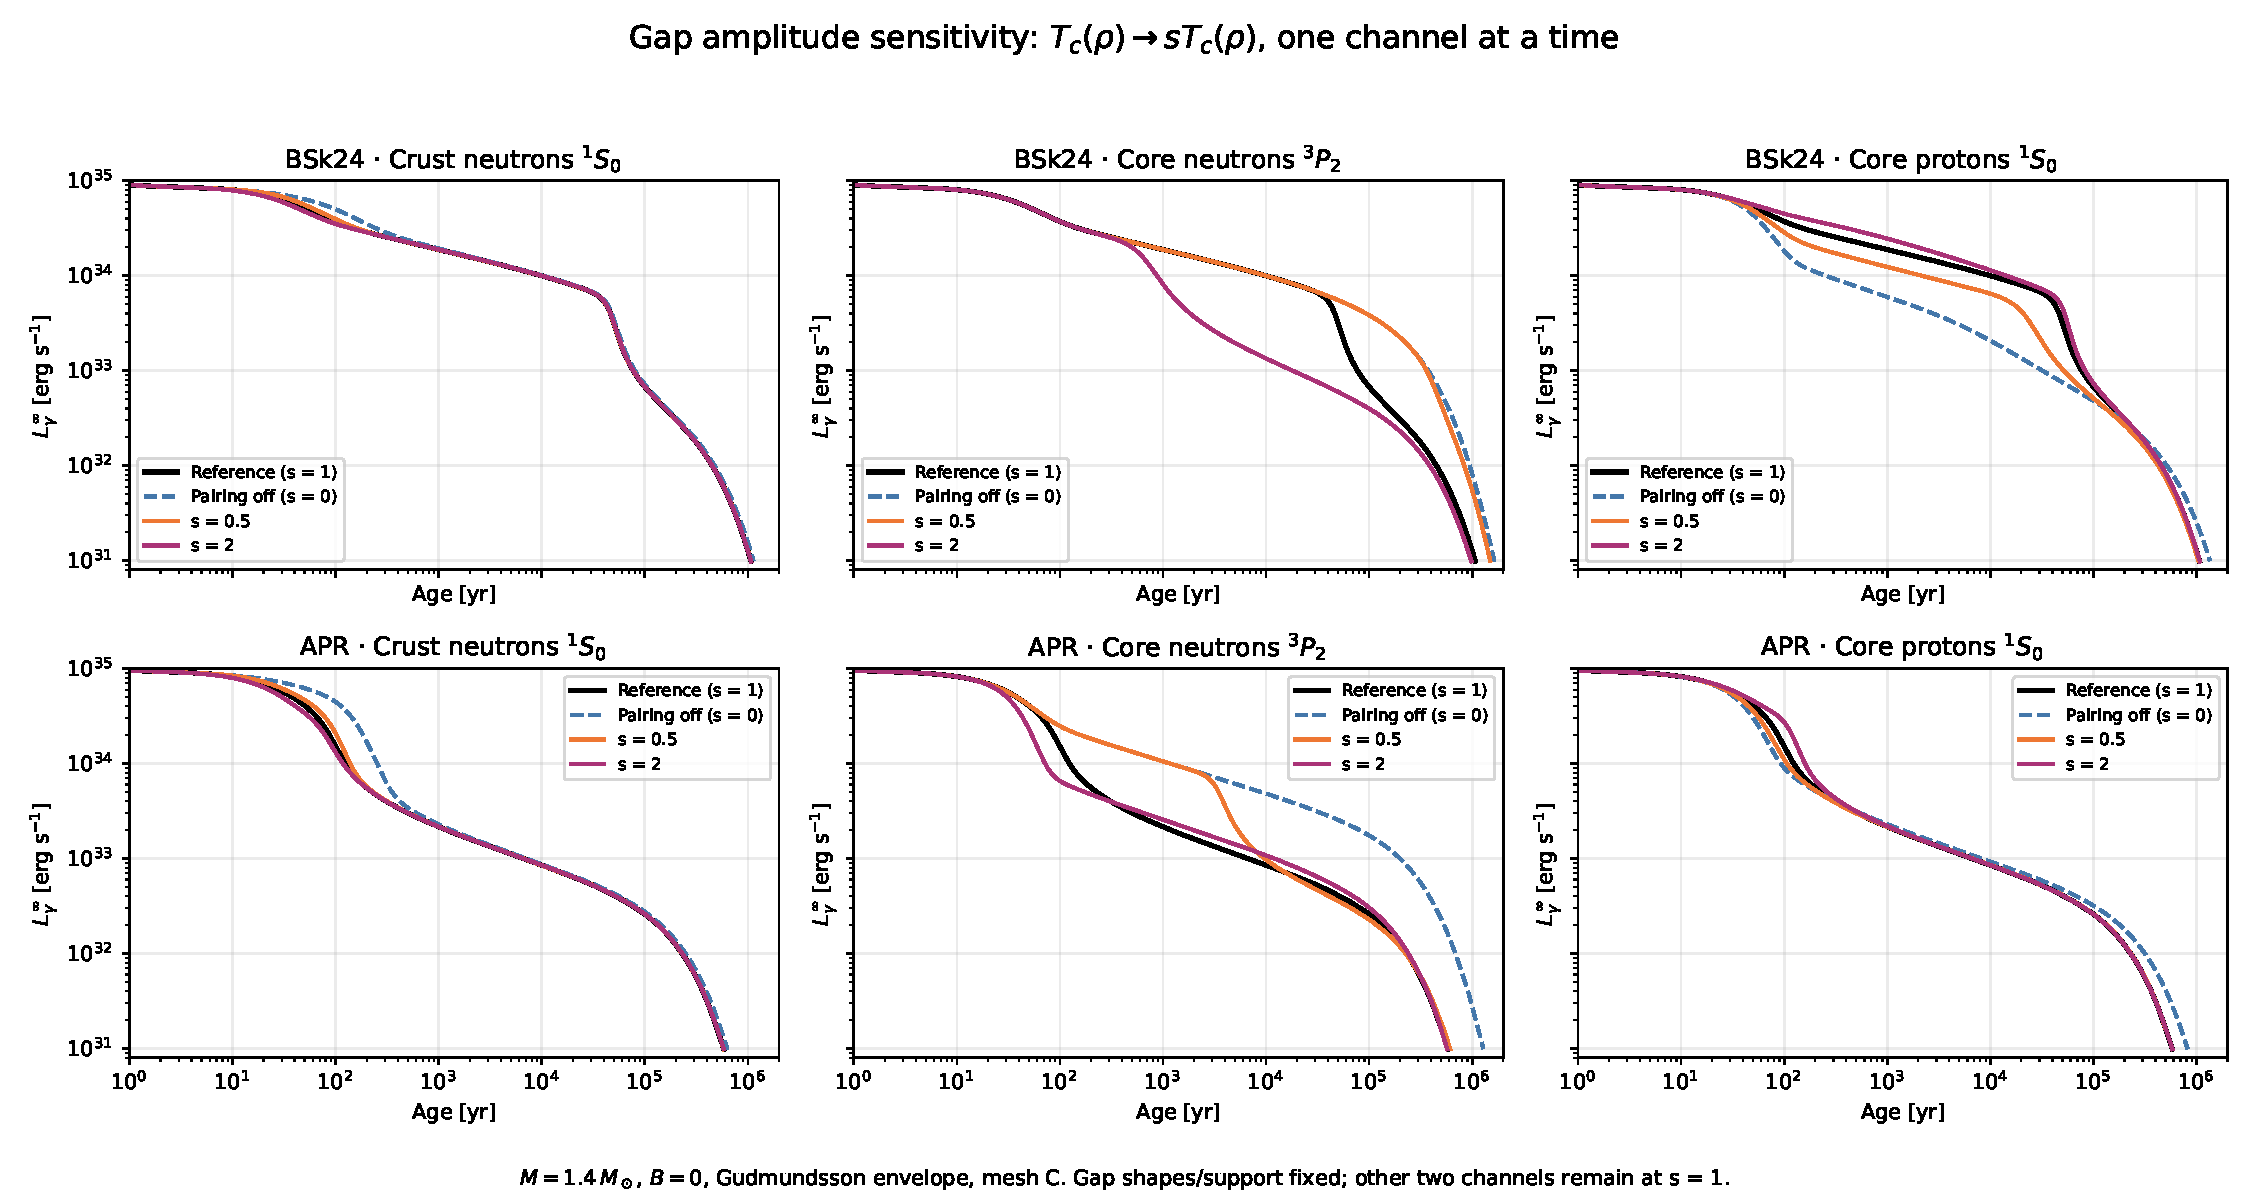
\includegraphics[width=\textwidth]{figures/gap_scan_luminosity.pdf}
\caption{One-channel gap-amplitude variations on fixed BSk24 (top) and DDFGOS(APR) (bottom) stellar backgrounds. Columns vary crustal neutrons, core neutrons, and core protons. Black is the reference; blue dashed switches the indicated pairing off; orange and purple multiply its $T_c$ by 0.5 and 2. The other two channels remain unchanged. The experiment varies amplitude only, not gap width, density support, or PBF response.}
\label{fig:gap-curves}
\end{figure*}

\begin{figure*}[t]
\centering
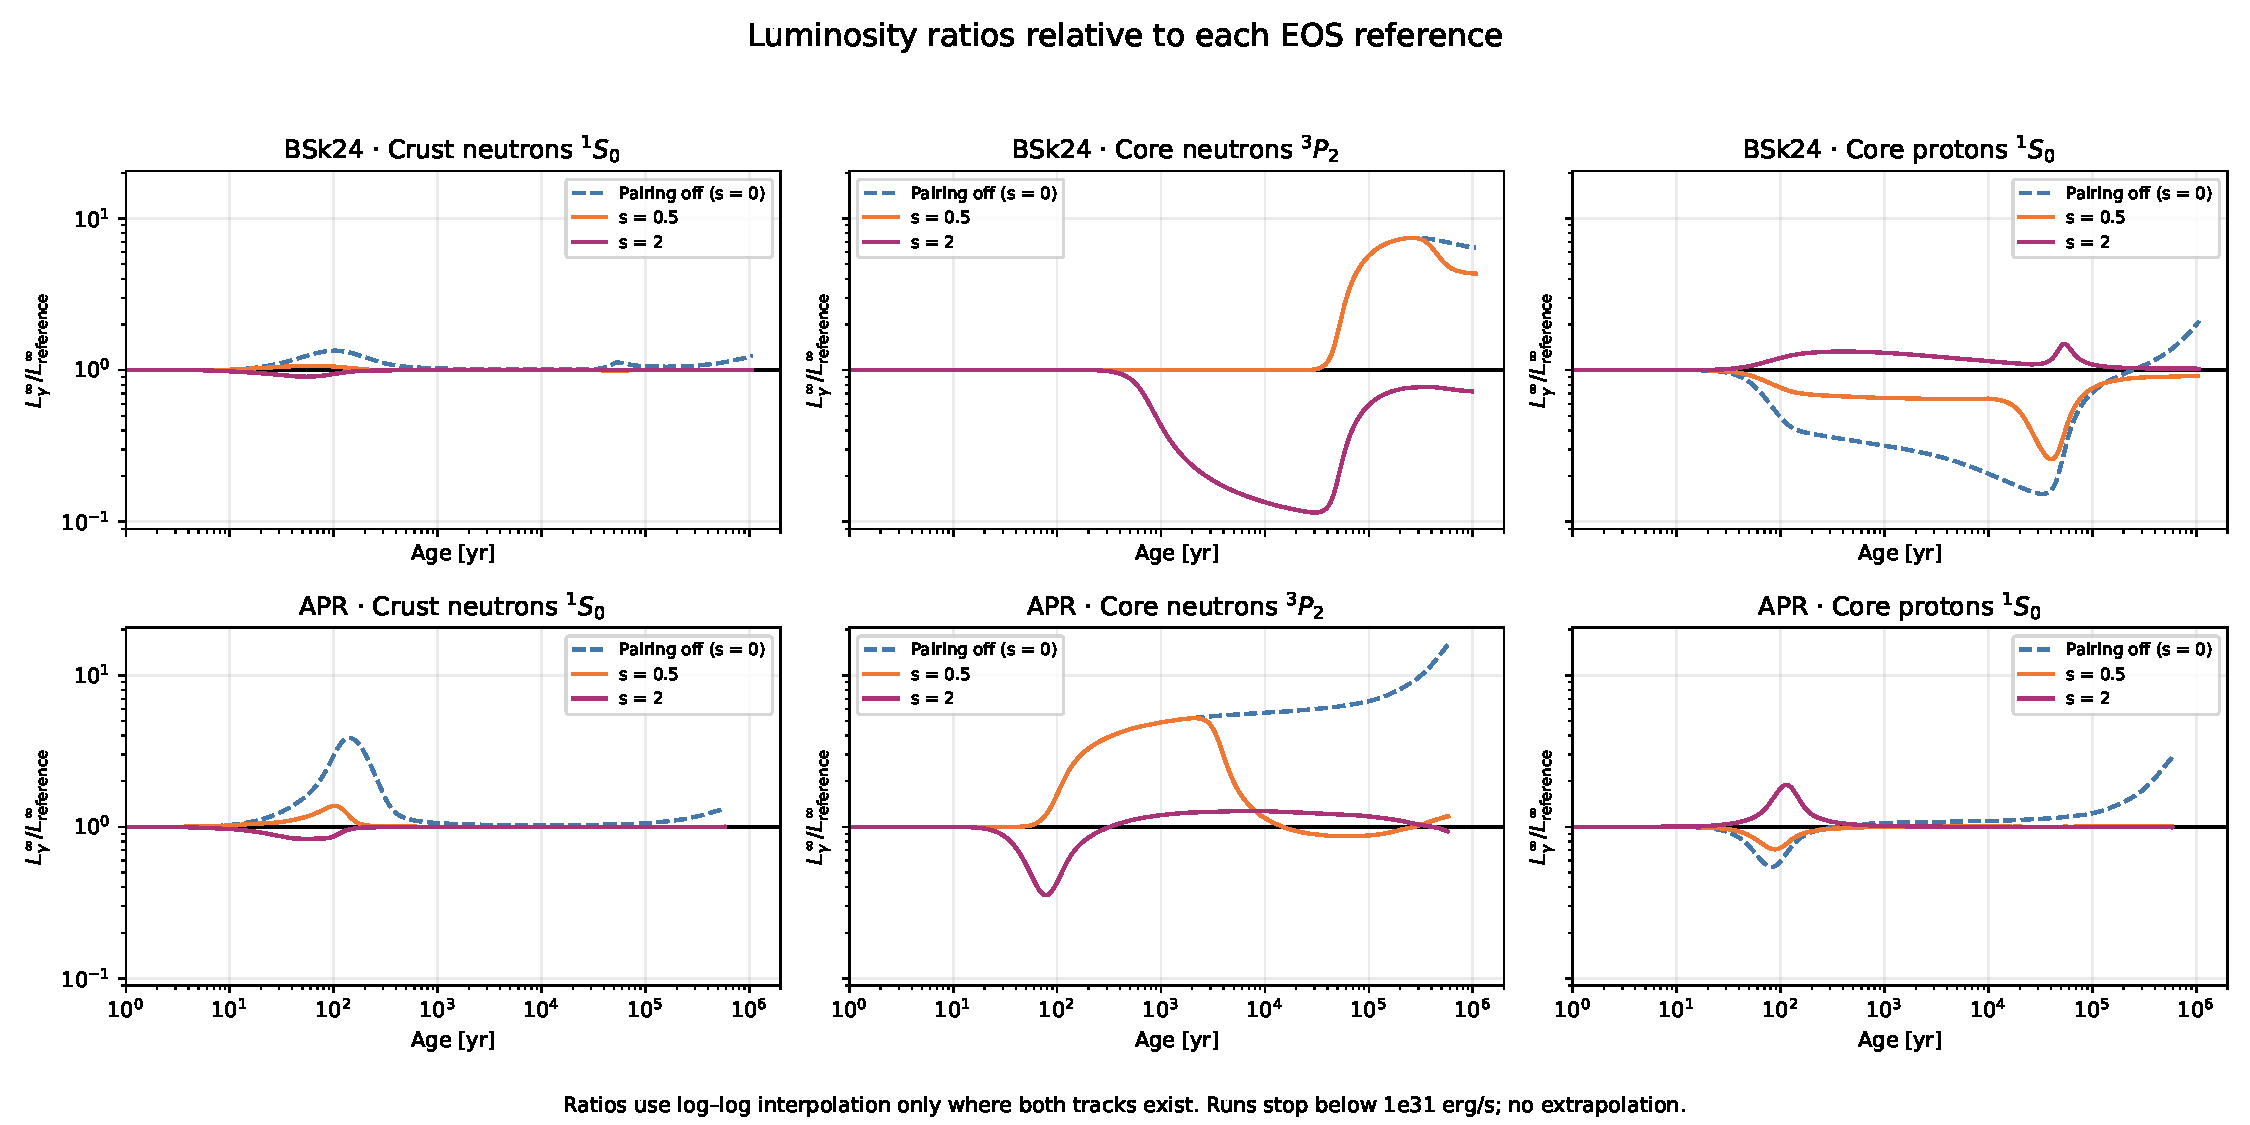
\includegraphics[width=\textwidth]{figures/gap_scan_ratios.pdf}
\caption{Ratios to the reference luminosity of each EOS for the same runs as Fig.~\ref{fig:gap-curves}. Ratios use logarithmic interpolation only over the common time interval of the two tracks. Strong changes in the timing of pairing transitions can give large temporary ratios even when late curves approach one another.}
\label{fig:gap-ratios}
\end{figure*}

\begin{table}
\caption{Luminosity ratios at $10^4$ yr relative to the reference of each EOS. Only the named channel is varied.}
\label{tab:gap-ratios}
\centering\small
\begin{tabular}{lrrr}
\toprule
Channel & $s$ & BSk24 & APR\\
\midrule
Core neutrons & 0 & 1 & 5.675\\
Core neutrons & 0.5 & 1 & 1.14\\
Core neutrons & 2 & 0.1345 & 1.269\\
Core protons & 0 & 0.2074 & 1.095\\
Core protons & 0.5 & 0.6479 & 1.004\\
Core protons & 2 & 1.144 & 1.001\\
\bottomrule
\end{tabular}
\end{table}

The maximum core-neutron critical temperature actually sampled by the reference stars is $4.057\times10^8$ K in BSk24 and $9.166\times10^8$ K in APR. These are stellar-profile maxima, not the maximum of the fitted gap over all momenta. The difference helps explain why the same amplitude variation has different consequences in the two EOSs. Table~\ref{tab:gap-ratios} quantifies selected changes. Both unmodified references reproduce the preceding five-EOS calculation to relative tolerance $10^{-10}$. The largest windowed energy-closure residual from 1 yr onward among the twenty runs is 0.116\%. This is an internal energy-accounting check, not an independent validation of the microphysics.

\subsection{Connecting global neutrino dominance to local emission}
\label{sec:neutrino-zones}
To distinguish local emissivity peaks from globally important losses, we record the luminosity of each neutrino process at every accepted time step,
\begin{equation}
 L_{\nu,i}^{\infty}(t)=\int_{\rm star}Q_i[\rho_b(r),T(r,t)]\,
 e^{2\Phi(r)}\,dV_{\rm proper}.
 \label{eq:process-luminosity}
\end{equation}
The dominant process is the largest individual $L_{\nu,i}^{\infty}$, not necessarily a majority of $L_\nu^\infty$. Its time intervals define the vertical shading in Fig.~\ref{fig:neutrino-zones}. This classification remains restricted to neutrinos even after the total neutrino luminosity falls below the photon luminosity.

For reference BSk24, three intervals occur over the plotted evolution: modified Urca, neutron--neutron bremsstrahlung, and core PBF. We choose accepted states nearest the geometric midpoint of each interval, so the markers are centred in logarithmic time. In the lower panels every emissivity is evaluated at the actual local temperature $T(r,t)=\Tinf(r,t)e^{-\Phi(r)}$, including thermal gradients. No isothermal profile is imposed for the diagnostic. Different contributions can dominate in different density layers; proper volume and redshift weighting determine the global result.

\begin{figure*}[t]
\centering
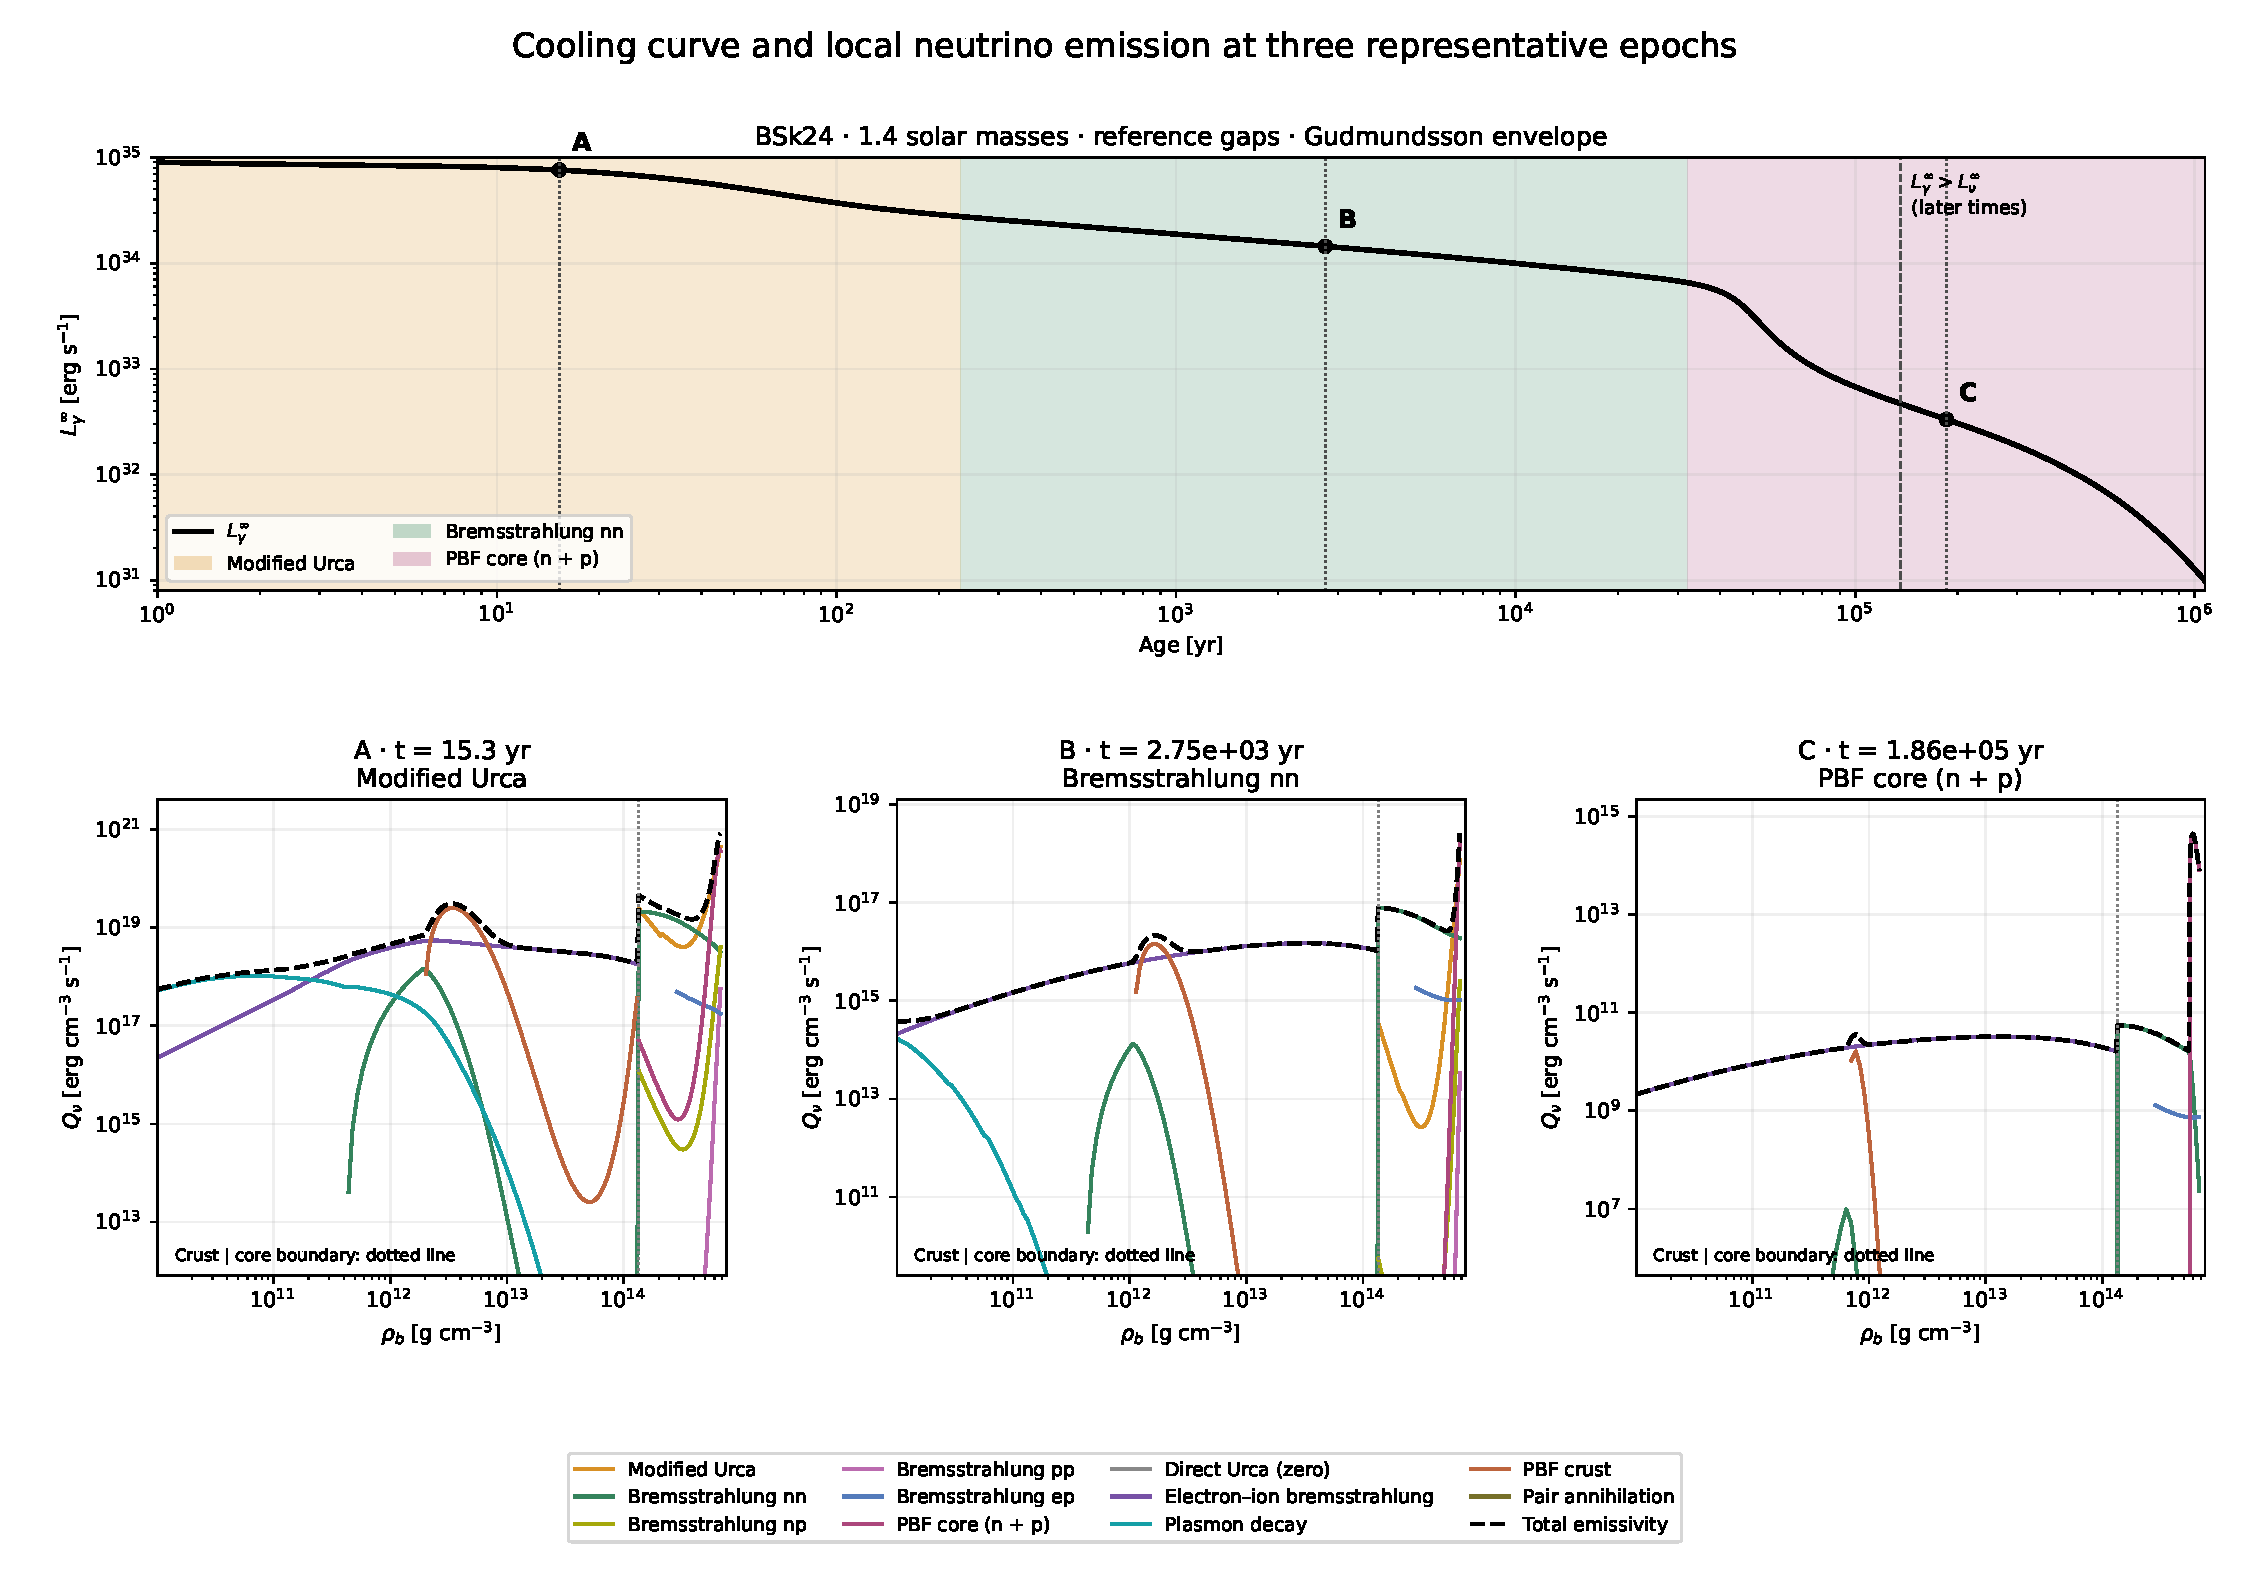
\includegraphics[width=\textwidth]{figures/BSk24_neutrino_zones.pdf}
\caption{Reference BSk24 cooling curve with shading by the leading integrated neutrino process (top), and local emissivities at three representative epochs (bottom). Colours identify the same processes throughout. The dashed black curve in each lower panel is the total emissivity; its vertical scale differs between panels. Dotted density markers locate the first core cell. Core PBF combines neutron and proton contributions. Direct Urca is zero for this star; zeros cannot appear on logarithmic axes. The upper dashed marker denotes the transition to photon-dominated total losses and does not change the neutrino-only shading.}
\label{fig:neutrino-zones}
\end{figure*}

\begin{table}
\caption{Representative BSk24 states. The final column is the leading process's fraction of the total neutrino luminosity at infinity.}
\label{tab:neutrino-zones}
\centering\small
\begin{tabular}{cllr}
\toprule
Point & Age [yr] & Process & Fraction [\%]\\
\midrule
A & 15.26 & Modified Urca & 49.36\\
B & 2750 & Brems.\ $nn$ & 60.98\\
C & 1.858e+05 & Core PBF & 99.91\\
\bottomrule
\end{tabular}
\end{table}

The two changes of leading neutrino process occur at approximately 231 yr and $3.20\times10^4$ yr. These boundaries are bracketed by accepted time steps and are not exact transition times. The total losses become photon-dominated at about $1.36\times10^5$ yr. Thus point C is PBF-dominated within the neutrino sector while $L_\gamma^\infty>L_\nu^\infty$. Reintegrating the three tabulated emissivity profiles with Eq.~\ref{eq:process-luminosity} reproduces each recorded process luminosity to relative tolerance $10^{-12}$. The snapshots therefore connect the global classification to the local emission consistently, without an additional thermal-evolution run with modified physics.

\clearpage
\section{Observations and the interpretation of cooling curves}
\begin{table*}
\caption{Evolution of the modelling questions. The right column states the proposed assessment strategy, not a completed result.}
\centering\small
\begin{tabularx}{\textwidth}{p{3.0cm}X X}
\toprule
Starting point & Subsequent development & Assessment required now\\
\midrule
Reaction inventory and minimal cooling (2001--2004) & Distinct nuclear-interaction, medium, and PBF-response revisions & Compare complete, named prescriptions with a common denominator.\\
Detailed thermal implementations (2008 era) & More consistent composition and updated gap catalogues & Match the EOS, lepton populations, mass definitions, and pairing assumptions.\\
Iron and layered accreted blankets & Diffusive mixtures and revised envelope synthesis & Vary light-element column and check fit domains; separate blanket from atmosphere.\\
Temperature--age diagrams & Larger samples, new cold sources, and secular cooling measurements & Preserve age and spectral alternatives, upper limits, and selection effects.\\
Code-to-code agreement & Independent energy accounting and modular implementations & Verify transcription, numerical convergence, and physical interpretation separately.\\
\bottomrule
\end{tabularx}
\end{table*}
\subsection{A curated sample rather than a universal cooling diagram}
The observational compilation of \citet{Vigano2013} was developed in a magneto-thermal context. For a non-magnetic review it is a starting source inventory, not a sample to import without selection. Magnetars, high-field objects with likely magnetic heating, and active accretors need separate treatment. A modest spin-down field alone does not establish an isothermal surface or the absence of internal magnetic effects.

\citet{Potekhin2020} provide a later compilation oriented towards cooling comparisons. A reproducible catalogue should record the primary observation and spectral analysis for each point, rather than cite only a changing web table. For this draft we retain the published compilations as guides; a homogenised, source-by-source table has not yet been constructed.

Each entry needs an age estimate and its method, a distance constraint, the thermal component and atmosphere assumptions, the emitting-area interpretation, a bolometric luminosity or upper limit, and the relevant confidence convention. Correlated alternatives should remain alternatives. Combining the age from one physical scenario with the luminosity from an incompatible spectral solution can create a source that no published analysis actually inferred.

\subsection{Age, emitting area, and limits}
Characteristic spin-down age need not equal the chronological age. Kinematic, remnant-based, or historical estimates are preferable when their assumptions are justified, but can also conflict. The correct response is to carry the competing age intervals through the interpretation, not to average them into an artificially precise value.

A thermal hot spot does not measure whole-surface cooling. If the colder remainder is undetected, a whole-surface upper limit depends on atmosphere, absorption, distance, and radius assumptions. X-ray band luminosity is also not synonymous with bolometric photon luminosity. These distinctions can move an inferred point more than a modest correction to a core reaction rate. As a methodological recommendation, conclusions should first be tested against the observational alternatives, before using the cooling curve to select a microscopic coefficient.

\subsection{Young cold sources and enhanced cooling}
\citet{Marino2024} identify young and cold isolated stars that challenge the cooling models explored in their study, including PSR~J0205+6449, PSR~B2334+61, and CXOU~J0852$-$4617. Their analysis is an important motivation for revisiting the microphysics rather than merely enlarging the list of candidate EOSs.

The inference must nevertheless be stated at the appropriate level. A source below a particular family of minimal-cooling curves excludes that family under its assumptions; it does not by itself identify nucleonic direct Urca, an exotic constituent, or a unique mass. Conversely, the availability of alternative prescriptions does not automatically explain a cold source. A proposed alternative must be calculated with consistent structure, pairing, and envelope assumptions and tested against the other observed stars.

\subsection{Cassiopeia A: secular cooling and response uncertainties}
The interpretations of \citet{Page2011,Shternin2011} connected the observed decline of the Cassiopeia~A neutron star to the onset of neutron superfluidity. This is a powerful example of how time-resolved observations can constrain a transition rather than only an integrated cooling history. It is also sensitive to atmosphere modelling, detector response, and absorption.

The cross-instrument study of \citet{Elshamouty2013} and the later HRC analysis of \citet{Zhao2025} show why the existence of a declining flux and the precise inferred temperature slope must be distinguished. The latter find an independent flux decline but smaller temperature-decline rates than those inferred from ACIS, with a dependence on the treatment of absorption. Consequently, a particular observed slope should not be used as an exact calibration of the PBF vertex. The gap profile, stellar structure, envelope, and response prescription remain coupled in the interpretation; \citet{Ho2015} illustrate this dependence in EOS-specific fits.

\subsection{Older warm stars}
Warm objects at late ages provide a complementary test of the residual heat capacity and the adopted envelope, but passive cooling is not guaranteed to remain sufficient. \citet{YakovlevPethick2004} discuss the wider cooling framework, while \citet{Potekhin2020} show the sensitivity of older sources to neutron pairing. A mismatch in this regime should not be repaired automatically by changing a neutrino rate that is already energetically subdominant. Heating and age uncertainties must be assessed before claiming evidence for a particular gap.



\section{Recommended practice and open issues}
A reproducible benchmark should retain a named EOS and its composition, explicit effective-mass definitions, both electron and muon populations, identified gap models, and a specified envelope relation. The conventional neutrino rates remain valuable as a reference because they are widely used and traceable. They should be accompanied by separately selectable alternatives where the literature motivates a different response or interaction model.

The highest-priority unresolved comparisons are the treatment of triplet PBF vertices, medium-modified Urca near its kinematic boundary, the consistency of effective masses across thermal and kinetic coefficients, and the observational consequences of envelope composition. The full coupled lepton conductivity and a carefully documented crustal transport prescription should complete the transport baseline. Detailed uncertainties in the crust must be judged against the evolutionary phase being studied.

No cooling prescription is selected solely because it improves agreement with one source. A credible interpretation must also account for warmer objects, avoid using the same physics twice, and state what the data actually constrain. The aim is not to eliminate alternative models from the review, but to make their assumptions and observational consequences sufficiently explicit that their merits can be assessed.

\section{Conclusions}
The framework established by the early reviews remains useful, but its modern implementation requires more than updated numerical coefficients. Composition and quasiparticle properties connect stellar structure to the thermal problem; weak-current conservation changes the interpretation of paired emission; nuclear medium effects introduce density-dependent alternatives; and the envelope and atmosphere connect the interior to different aspects of the observations.

The controlled calculations reinforce the need to separate established transcription corrections, numerical interface choices, and competing physical models. Changing the amplitude of the same core-neutron gap has different consequences in BSk24 and APR because each stellar structure samples a different part of its density dependence. Integrated process luminosities and local emissivity profiles provide complementary diagnostics; a late neutrino-dominant process can already be subdominant to photons in the total energy balance. These preliminary experiments do not select a microscopic model. Further comparisons must vary gap shape and weak response independently, assess spatial convergence and APR crust composition, and retain observational alternatives in a curated source table.

\begin{acknowledgements}
Author contributions, funding, and acknowledgements will be added after agreement on the manuscript scope and author list.
\end{acknowledgements}
\bibliographystyle{aa}
\bibliography{references}

\begin{appendix}
\section{Source map for implementation and review}
\label{app:sources}
The main text intentionally avoids reproducing extensive fits. The neutrino benchmark is \citet{Yakovlev2001}: Sect.~3.3 for direct Urca, Eqs.~(140)--(142) for modified Urca, Eqs.~(165)--(167) for nucleon bremsstrahlung, and the superfluid sections for reduction functions and the original PBF expressions. The paired-matter response must then be updated with explicit reference to \citet{Leinson2006,Page2009,Leinson2010}, rather than silently changing the older formula.

For modified nuclear rates, use the published version of \citet{Bottaro2024}; for the distinct intermediate-state enhancement use \citet{Shternin2018}, including its stated approximation limits. Equation-level disagreements raised by our working code audit are not presented here as established errata of those papers. They require a dedicated check of the published expressions and conventions before inclusion in a review.

For transport, the principal comparisons are \citet{Potekhin1999,Shternin2006,Shternin2007,Baiko2001}. Routine names and release dates should be archived with the actual software version; they are not substitutes for physical references. Envelope expressions should be traced to \citet{Gudmundsson1983,Potekhin1997,Beznogov2016,Beznogov2021} and compared at the same base density and gravity convention.


\section{Cold-EOS table handling and consolidated interface choices}
\label{app:eos-tables}
The original CompOSE tables are archived unchanged. All omissions described here belong to the interpolation reader and apply to composition, effective masses, pairing information, and thermodynamic fields together. Sorting pressure independently would break their correspondence. In density order, a stable homogeneous branch has increasing pressure; pressure decreases when following the star outward.

The cold tables supply both $P/n_b$ and the scaled baryon chemical potential $\mu_b/m_n-1$, as well as the energy per baryon. For neutral, neutrino-free matter in beta equilibrium at $T=0$, the identity $\mu_b=(\varepsilon+P)/n_b$ supplies a consistency check. A Maxwell construction requires equal pressure and baryon chemical potential on the two locally neutral phases. The existence of tabulated chemical potentials does not guarantee sufficient sampling of both branches to locate coexistence precisely.

\begin{figure*}[t]
\centering
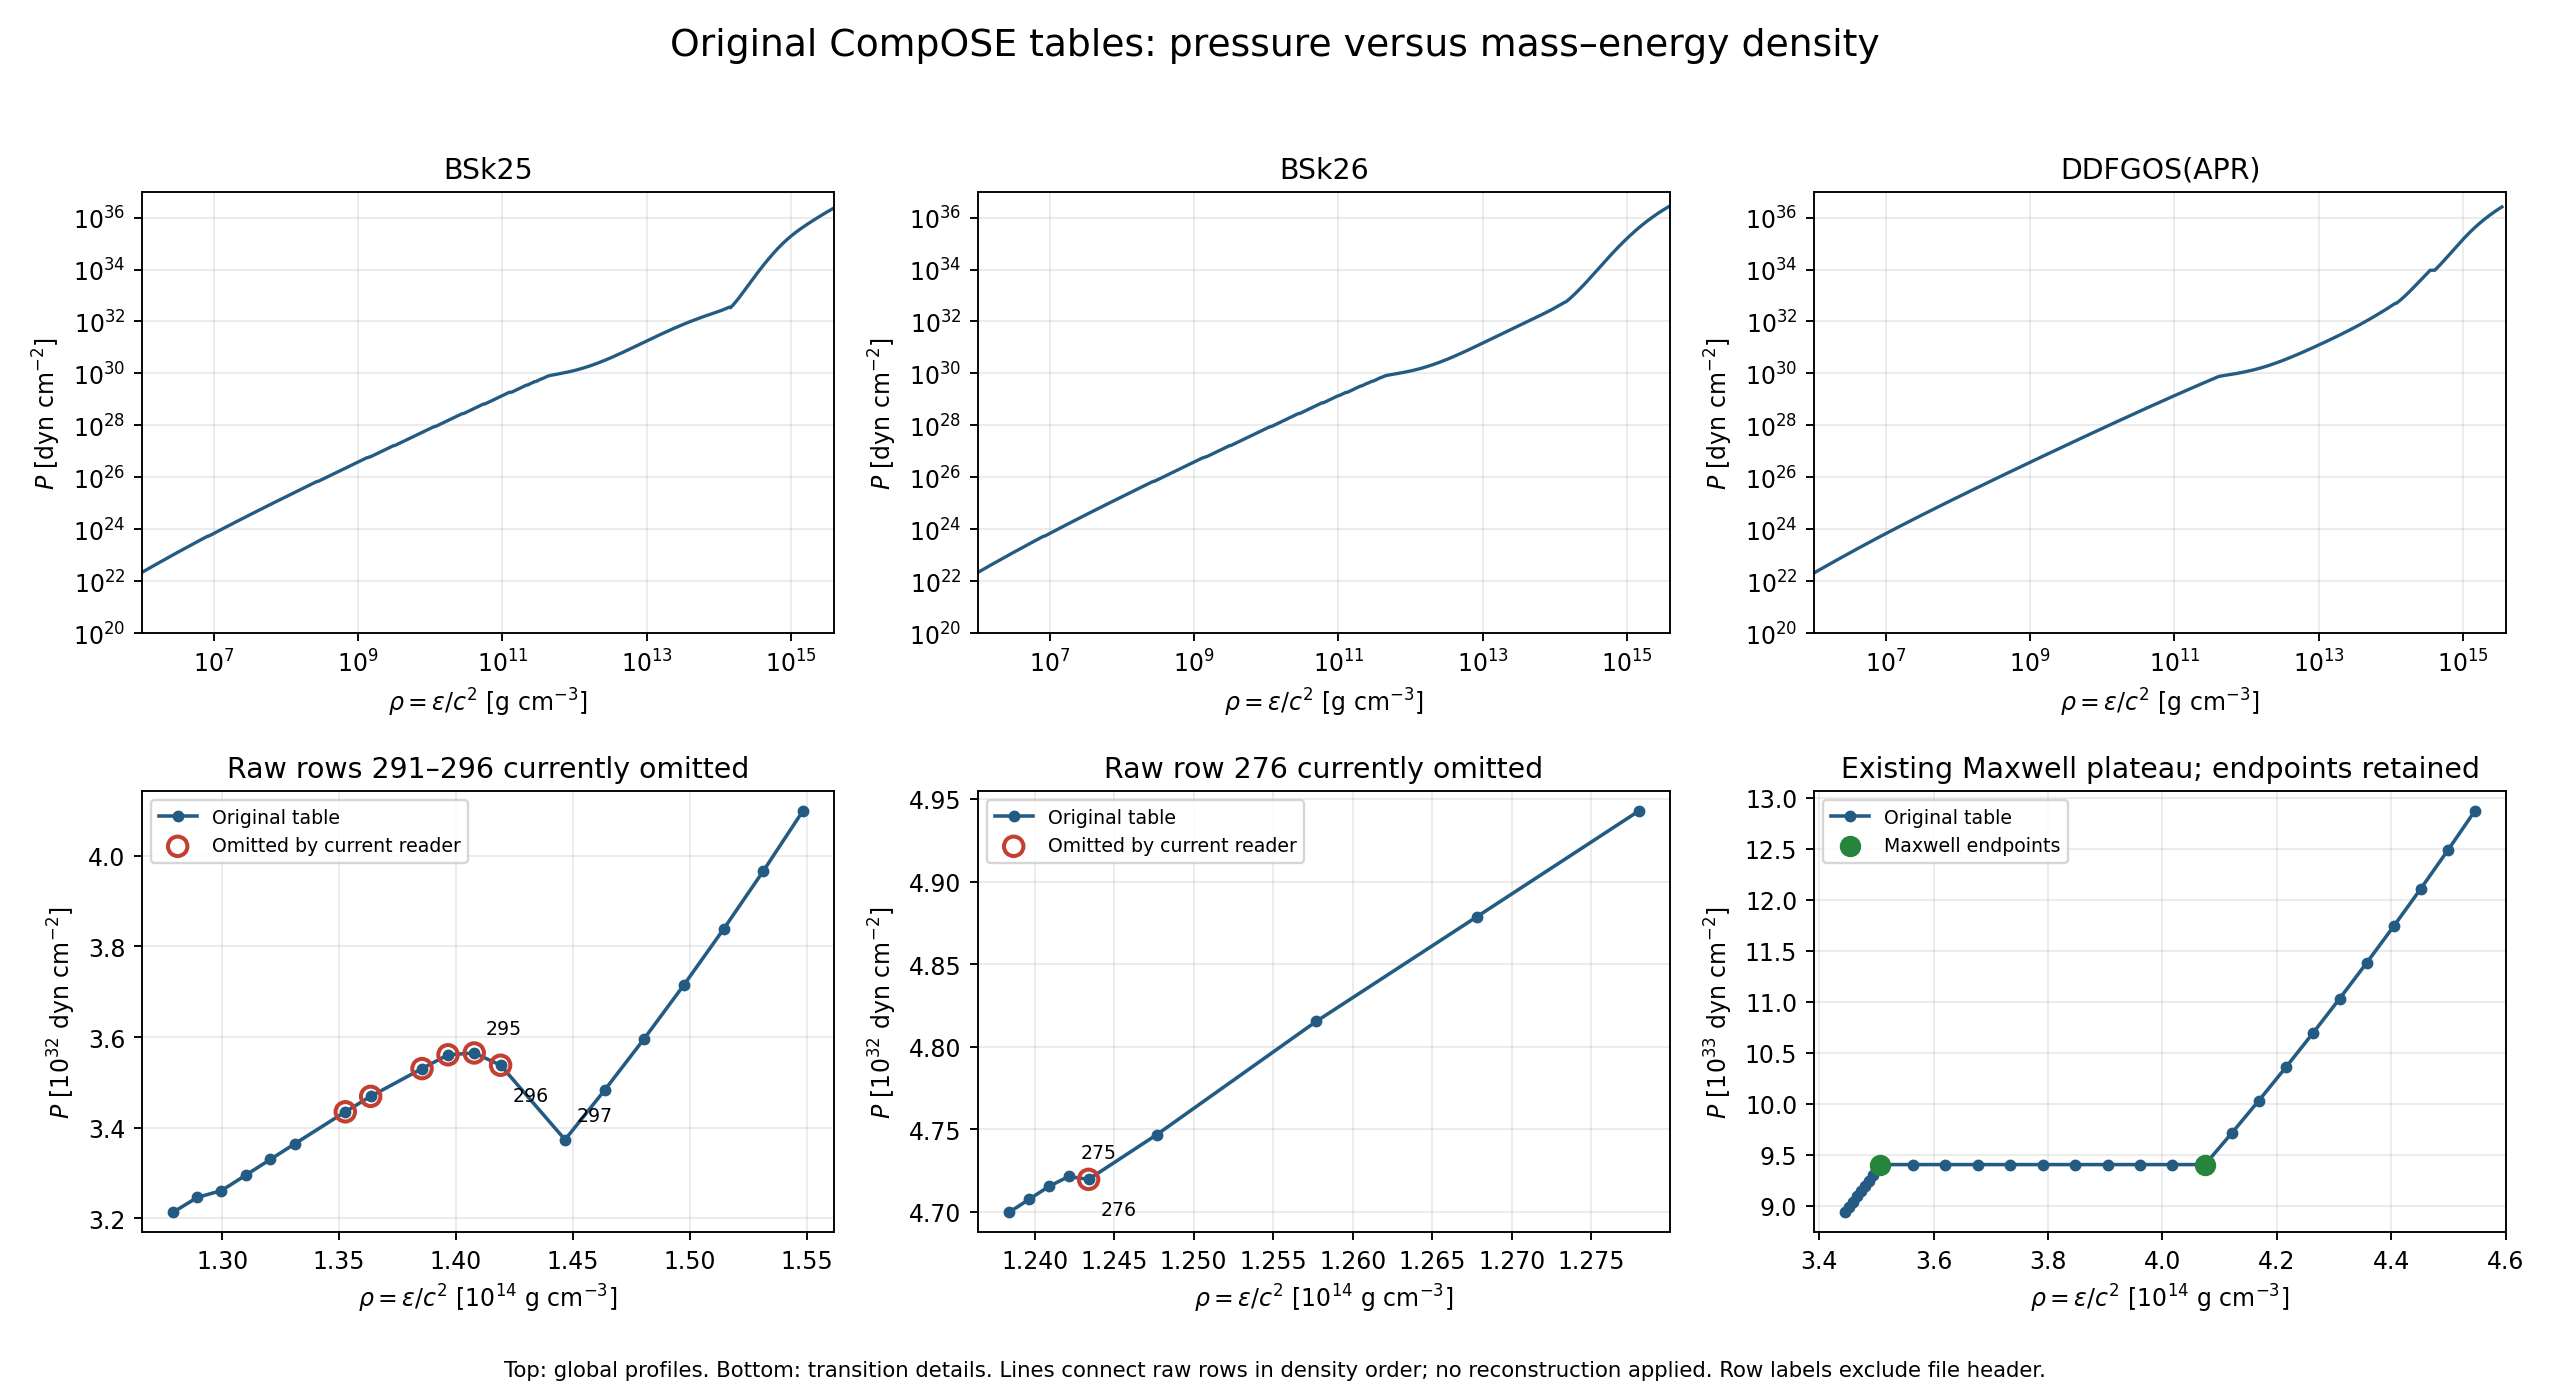
\includegraphics[width=\textwidth]{figures/eos_pressure_profiles.png}
\caption{Original table pressure versus mass--energy density $\rho=\varepsilon/c^2$, distinct from $\rho_b$ used in the microphysics. Top: global profiles. Bottom: transition details for BSk25, BSk26, and DDFGOS(APR). Red circles mark rows omitted by the reader; green points mark the two retained Maxwell endpoints of APR. Lines connect rows in their original density order. Labels count data rows, excluding file headers.}
\label{fig:eos-pressure}
\end{figure*}

\subsection{BSk25 and BSk26 pressure reversals}
The PCP(BSk25) package is CompOSE entry 257, and the DDFGOS(APR) package is entry 327; the archived provider files specify their full source provenance.\footnote{\texttt{https://compose.obspm.fr/eos/257} and \texttt{https://compose.obspm.fr/eos/327}.} In BSk25, the final crust rows overshoot the first homogeneous-core pressure and then turn down. The adopted reader omits crust data rows 291--296 and connects retained crust row 290 directly to core row 297. The latter has $n_b=0.0855534$ fm$^{-3}$ and $P=0.2105624368$ MeV fm$^{-3}$.

After comparing both $P(\rho)$ and $P(\mu_b)$, we consolidate this connection as the discrete approximation to Maxwell coexistence adopted at the resolution of the supplied table. It retains the first core state and removes the pressure overshoot without extrapolating unprovided phase branches. It does not enforce exact equality of $P$ and $\mu_b$ between the two retained rows, determine an exact coexistence crossing, or introduce a reconstructed constant-pressure plateau. It should therefore be reported as an adopted interface prescription, not a provider-issued thermodynamic correction.

For BSk26, data row 276 lies approximately 0.037\% below the pressure of row 275. Omitting only row 276 restores monotonicity; this single-row omission is also adopted. BSk22 and BSk24 have no pressure inversions in the supplied tables. The original BSk25 local reversal is substantially larger: the accumulated decrease from its pressure maximum to the first core row is approximately 5.37\%.

\begin{figure*}[t]
\centering
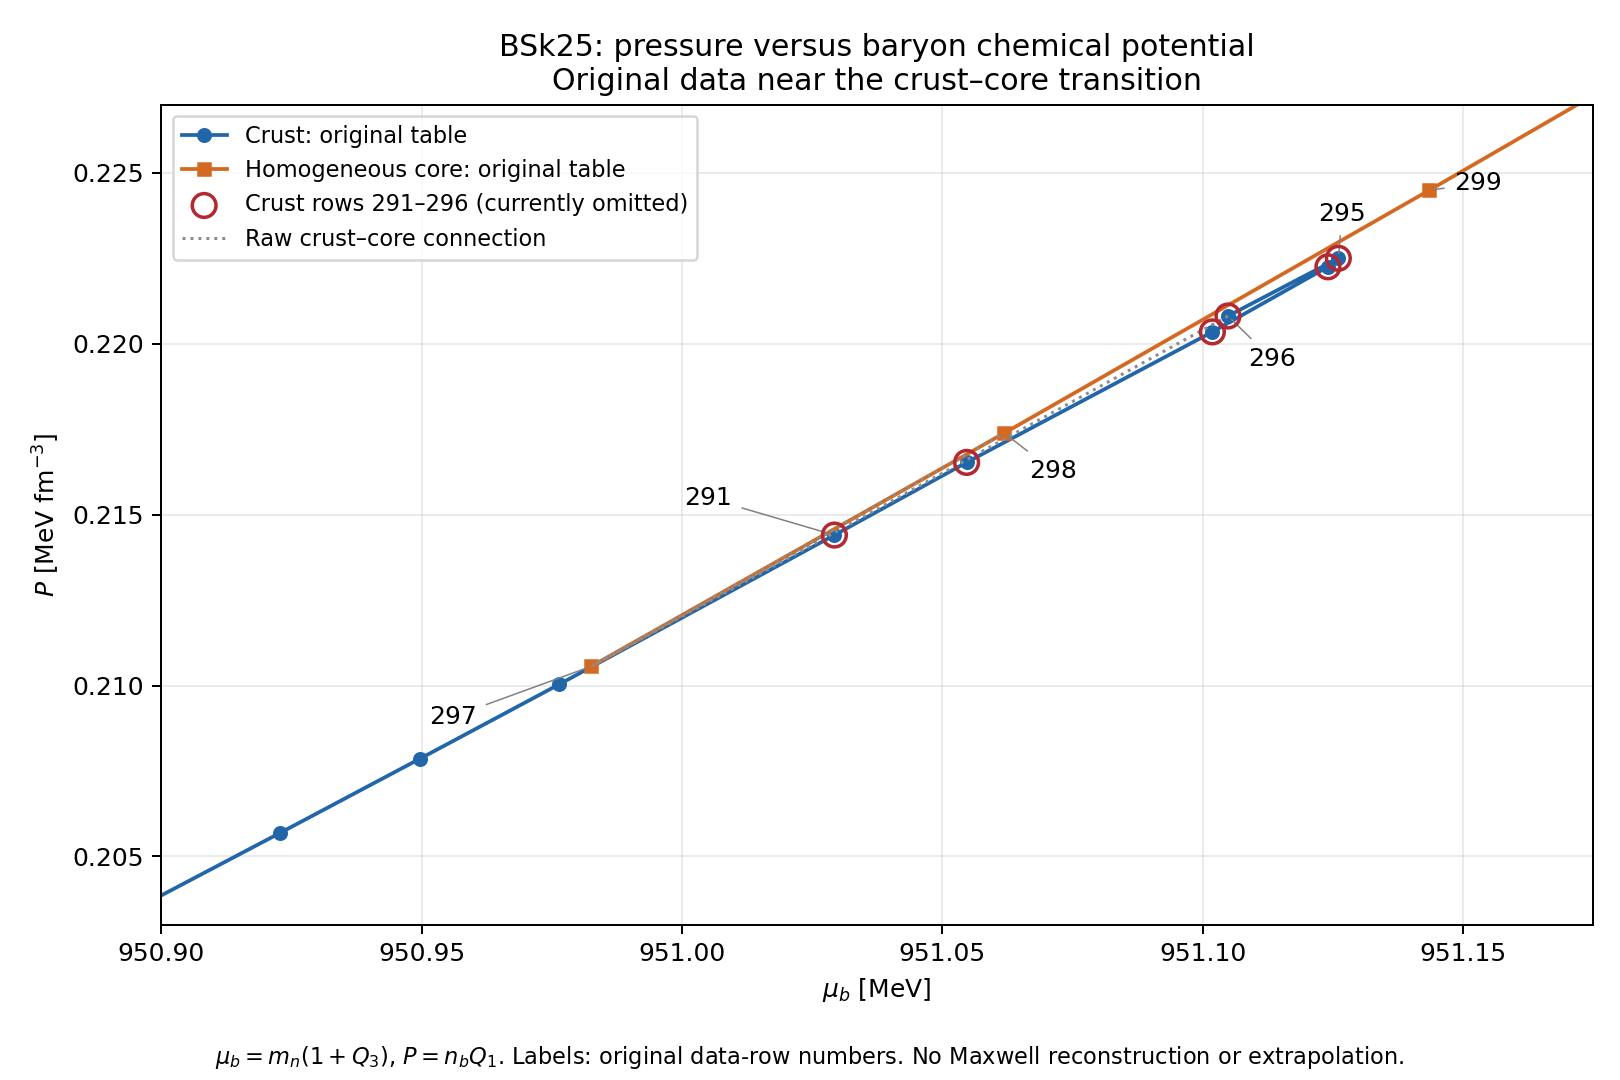
\includegraphics[width=0.85\textwidth]{figures/BSk25_pressure_mu_b.png}
\caption{Original BSk25 crust and homogeneous-core branches in the pressure--baryon-chemical-potential plane. Red circles identify crust rows 291--296; the dotted grey connector follows the original transition between phase tables and is not a physical coexistence branch. The adopted discrete connection retains rows 290 and 297. No Maxwell crossing has been solved or extrapolated in this plot.}
\label{fig:eos-mu}
\end{figure*}

\subsection{The existing APR Maxwell interval}
APR rows 1886--1896 already describe a constant-pressure transition at $P=5.8692415398$ MeV fm$^{-3}$. Its endpoint baryon densities are 0.2047519151 and 0.2369174514 fm$^{-3}$; the endpoint chemical potential is $\mu_b=989.464754$ MeV on both sides. The reader retains both endpoints, omits only interior rows 1887--1895, and preserves the finite density jump. Interpolation does not create a finite shell of intermediate mixed states, and the cooling mesh places a face at the discontinuity.

A separate APR issue remains open: the tabulated inner-crust fractions and cluster quantities do not satisfy the composition mapping assumed by the cooling code. Retaining the provider's electron and free-neutron fractions gives provisional crustal thermal properties, not a validated correction to that mapping. Good mass--radius agreement and accurate energy closure do not resolve this composition question. The structural phase transition is retained, but no additional pion-condensate neutrino channel has been introduced in this common-microphysics comparison.

\section{Status of the working draft}
This manuscript combines a literature-based discussion with preliminary controlled cooling experiments, not a completed meta-analysis. It does not introduce a new emissivity derivation, reproduce copyrighted figures, or report a new statistical fit to the observations. The accompanying editorial notes list the remaining equation-level checks, observational provenance work, and further numerical comparisons. The EOS and gap experiments are internal model comparisons, not an independent validation of all adopted microphysics. Author names and affiliations are placeholders. Literature selected during preparation includes work through 2025; completeness of the 2026 literature has not been established.
\end{appendix}
\end{document}
